\documentclass[a4paper, 11pt]{article}
\usepackage{amsmath}
\usepackage{amssymb}
\usepackage[T1]{fontenc}
\usepackage[utf8x]{inputenc}
\usepackage{lmodern}
\usepackage{graphicx}
\graphicspath{ {./images/} }
\usepackage[english]{babel} 
\usepackage{natbib}
\usepackage{cite}
\usepackage[parfill]{parskip}
\usepackage{enumerate}
\usepackage{float}%for image positions
\usepackage{hyperref}
\hypersetup{
  colorlinks,
  citecolor=black,
  filecolor=black,
  linkcolor=black,
  urlcolor=black
}
\usepackage{amsthm}
\newtheorem{theorem}{Theorem}[section]
\newtheorem{lemma}[theorem]{Lemma}
\newtheorem{proposition}[theorem]{Proposition}
\newtheorem{axiom}[theorem]{Axiom}
\newtheorem{invariant}[theorem]{Invariant}
\newtheorem{breakpoint}[theorem]{Breakpoint}
\newtheorem{problem}{Problem}
\newtheorem{definition}{Definition} 
\usepackage{algorithm}
\usepackage{algpseudocode}
\usepackage{pifont}
\usepackage{multirow,array}
\usepackage{centernot}
\usepackage{listings}
\usepackage{xcolor}

\usepackage{graphicx}

\newcommand\mymapsto{\mathrel{\ooalign{$\rightarrow$\cr%
      \kern-.15ex\raise.275ex\hbox{\scalebox{1}[0.522]{$\mid$}}\cr}}}

\lstdefinestyle{base}{
  language=C,
  emptylines=1,
  breaklines=true,
  basicstyle=\ttfamily\color{black},
  moredelim=**[is][\color{red}]{@}{@},
}

\usepackage{comment} % enables the use of multi-line comments (\ifx \fi) 
\usepackage{lipsum} %This package just generates Lorem Ipsum filler text. 
\usepackage{fullpage} % changes the margin

\begin{document}
\noindent
\large\textbf{Assignment 1  - Extra non-submission tasks} \hfill \textbf{Kim Hammar} \\
\normalsize ID2204 \hfill  \textbf{Mallu} \\
Constraint Programming \hfill Due Date: 7 April 2017\\
\section*{Search Heuristics}
Can you find a better heuristic than first-fail for the following crypto arithmetic puzzle?

$$DONALD + GERALD = ROBERT$$

Comparison between first-fail min-value (ffminv), first-fail max-value (ffmaxv), first-fail split-max(ffsmax), first-fail split-min (ffsmin).
\begin{center}
  \begin{tabular}{ | l | l | l | p{7cm} |}
    \hline
    \textbf{Search Heuristic} & \textbf{nodes} & \textbf{failures} \\ \hline
    ffminv & 178 & 87 \\\hline
    ffmaxv & 50 & 23 \\\hline
    ffsmax & 50 & 23 \\\hline
    ffsminv & 180 & 87 \\\hline
  \end{tabular}
\end{center}
First-fail max-value and First-fail split-max are the best heuristics I've found. The main difference is that when picking max-value instead of min the failed sub-trees is a lot smaller. I.e trying the larger values first give more constraints and more propagation possible.

\section*{Is Propagation Compositional?}
Assume that $A, B, C,$ and $X$ are finite domain variables and that you are given
the following statement:

$$A+B+C+B = X$$

It looks intuitive that you can transform this into

\texttt{IntVar U}\\
$A+B = U$\\
$U+B+C = X$

Implement the two programs and analyze what is different.

The two solution sets are identical which is shown by the program. Does this mean propagation is compositional?

Is there any other aspect in which they compute differently? In which aspect?

Propagation is not compositional, propagations communicate through the variables values and assignments. 

Yes they result in different search trees despite the fact that they are using the same search-heuristics (branching strategies):

First we have script $S1$ which models $A+B+C+B = X$ where $D_A = D_B = D_C = D_X = \{1,2,3,4,5\}$
\begin{figure}[H]
  \begin{center}
    \scalebox{0.90}{
      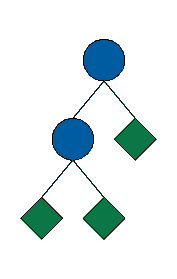
\includegraphics{first_fail_valmin_s1.pdf}
    }
    \caption{First-fail Minimum-value for Script S1}
    \label{fig:ffvms1}
  \end{center}
\end{figure}

Second we have script $S2$ which models $A+B = U; U+B+C = X$ where $D_A = D_B = D_C = D_X = D_U = \{1,2,3,4,5\}$
\begin{figure}[H]
  \begin{center}
    \scalebox{0.90}{
      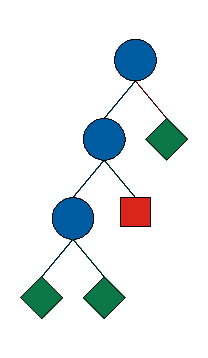
\includegraphics{first_fail_valmin_s2.pdf}
    }
    \caption{First-fail Minimum-value for Script S2}
    \label{fig:ffvms2}
  \end{center}
\end{figure}

What is happening?

In S1 we only post one constraint that will create propagators for that single constraint while in S2 there are two constraints posted. In the search tree of S2 the propagator for $A + B = U$ is executed first which results in interleaving of constraint propagation and variable assignment until the constraint is satisfied, in particular the assignments $A = 1, B = 2, U = 3$ is tried which leads to a (red) failed node since that means that there are no satisfying assignments for $C$ and $X$ that gives $U+B+C = X$. This is because $U+B=5$ and the maximum value of X is $5$ and the minimum value of $C$ is 1.

In S1 already before any assignment is made constraint propagation can infer that $B$ must be 1. This is the main difference. In S2 the constraint propagation were not able to resolve this initially since just looking at the constraint $U+B+C=X$ B could be other things than 1. But if the constraint propagation were able to consider both constraint simultaneously it would find out that $B$ could not be something else than 1, looking at each constraint in isolation $B$ does not have to be only 1.

\section*{Search Heuristics for N-Queens}
\subsection*{First-Fail Minimum-Value}
The standard first-fail heuristic is the first-fail minimum-value heuristic, the search tree for it is shown in the figure below. 
\begin{figure}[H]
  \begin{center}
    \scalebox{0.90}{
      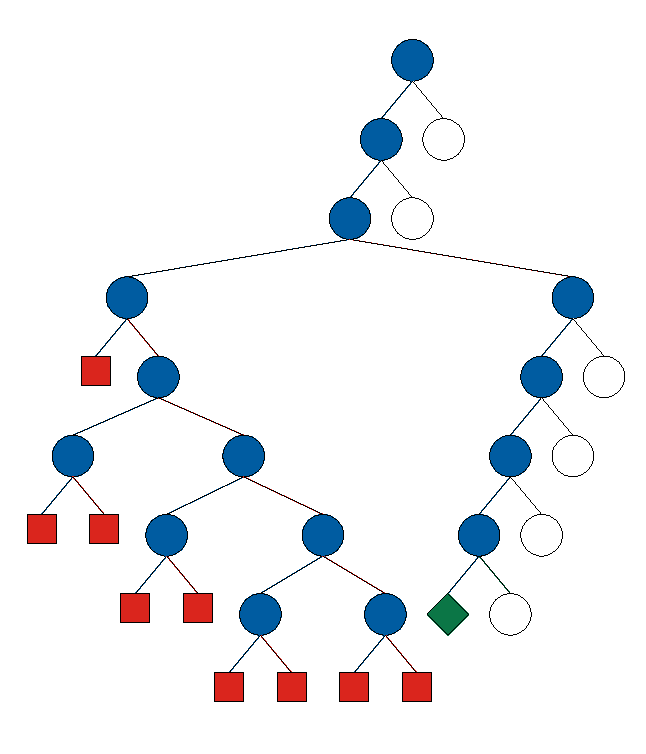
\includegraphics{first_fail_valmin_10.pdf}
    }
    \caption{First-fail Minimum-value for queen problem instance of size 10}
    \label{fig:ffvm10}
  \end{center}
\end{figure}
It visits 25 nodes and 9 failures before finding the first solution.

\subsection*{First-Fail Median-domain-value}
\begin{figure}[H]
  \begin{center}
    \scalebox{0.90}{
      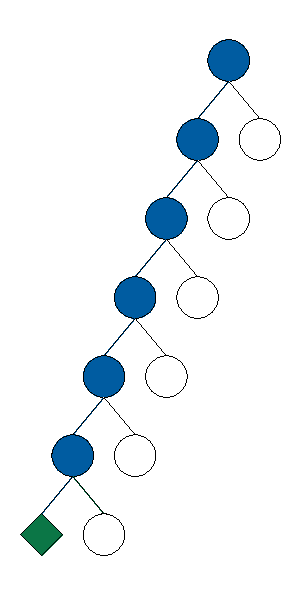
\includegraphics{first_fail_med_10.pdf}
    }
    \caption{First-fail Median-value for queen problem instance of size 10}
    \label{fig:ffmv10}
  \end{center}
\end{figure}
The search visits 7 nodes and 0 failures before finding the first solution.

\subsection*{Knight-move heuristic (min-min median-domain-value)}
\begin{figure}[H]
  \begin{center}
    \scalebox{0.90}{
      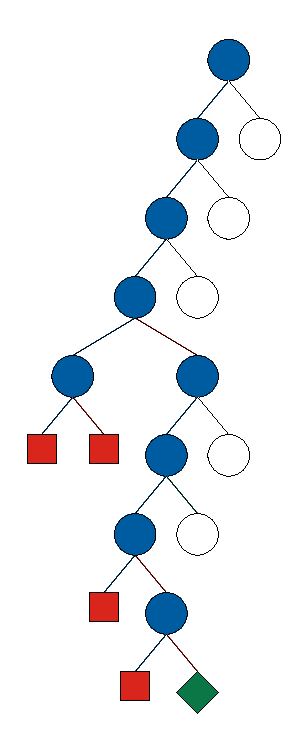
\includegraphics{knight_move_med_10.pdf}
    }
    \caption{Knight-move Median-value for queen problem instance of size 10}
    \label{fig:kmm10}
  \end{center}
\end{figure}
This search visits 14 nodes and 4 failures before finding the first solution.
\subsection*{Knight-move heuristic (min-min val-min)}
\begin{figure}[H]
  \begin{center}
    \scalebox{0.60}{
      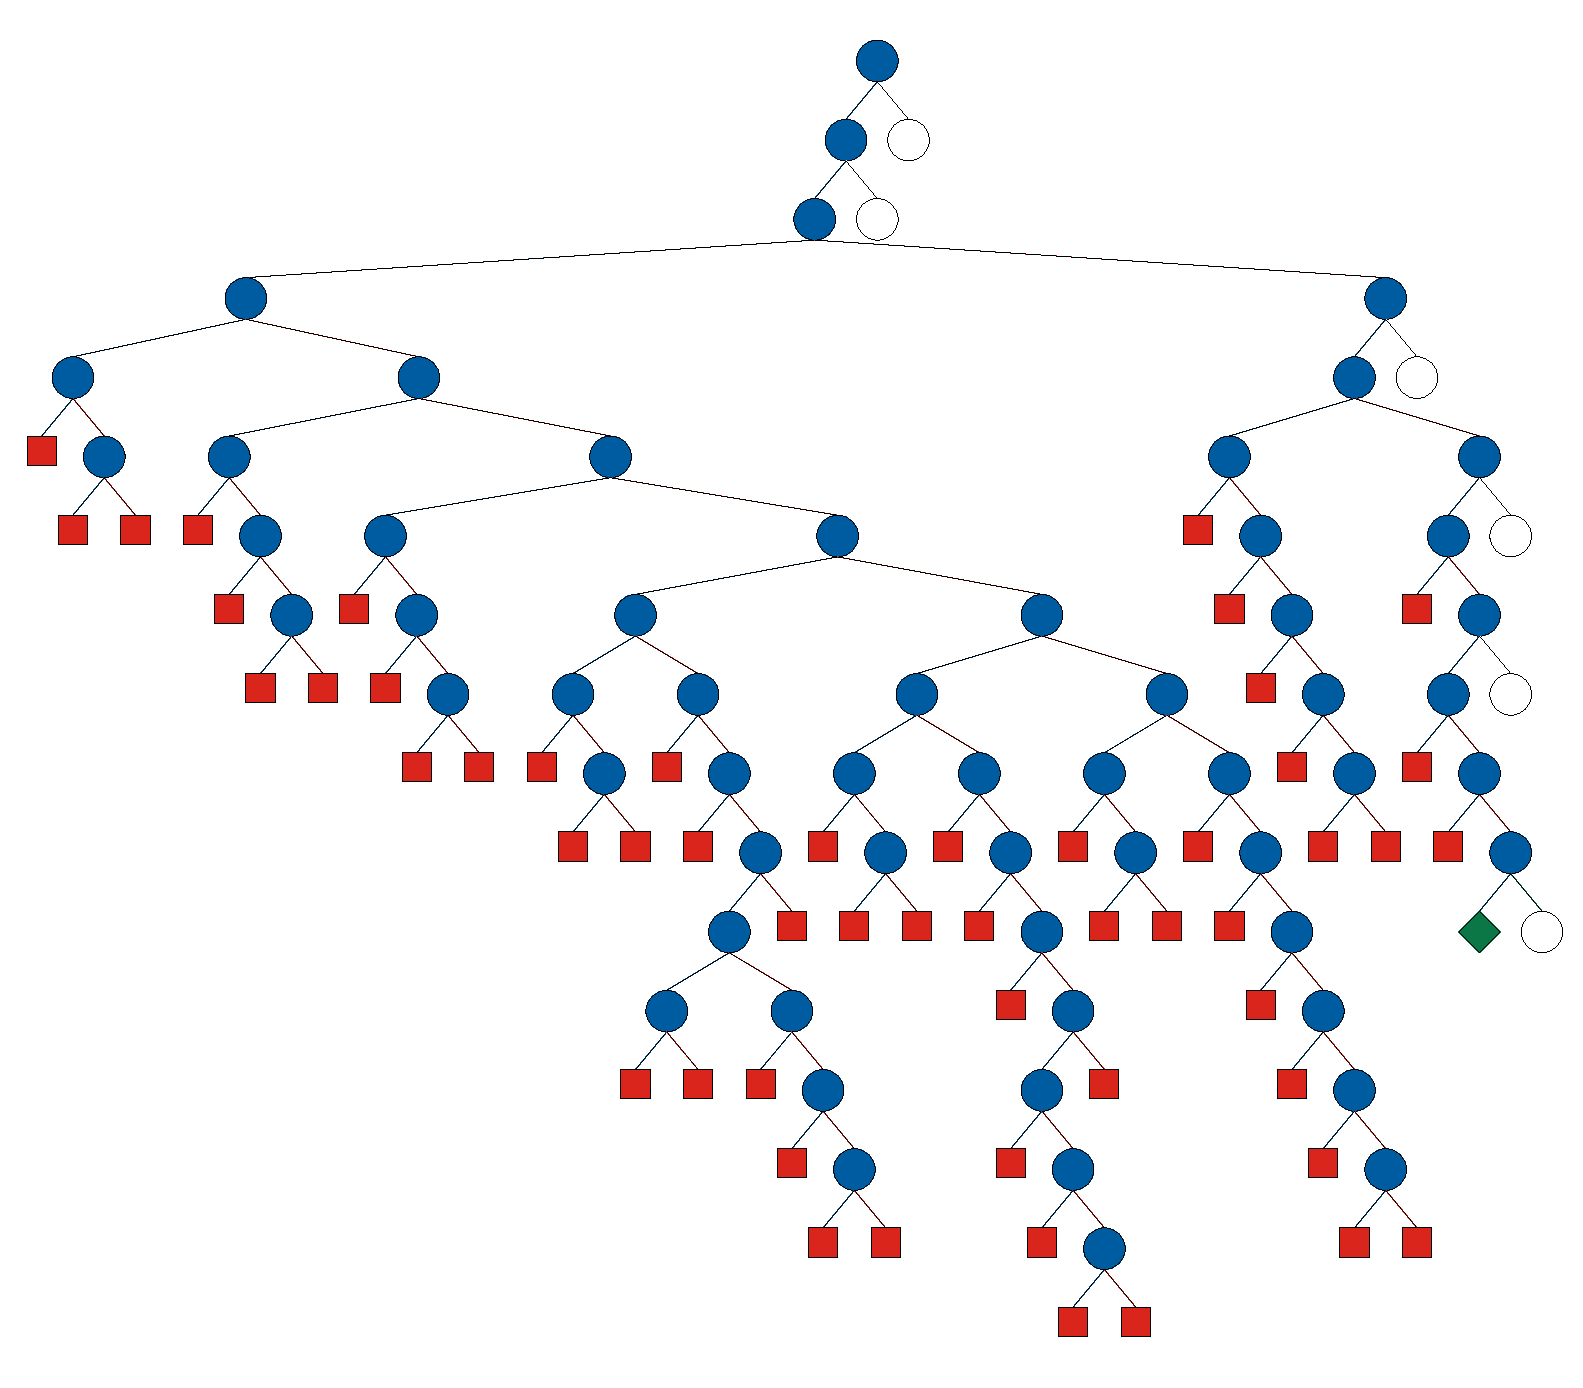
\includegraphics{knight_move_valmin_10.pdf}
    }
    \caption{Knight-move minimum-value for queen problem instance of size 10}
    \label{fig:kmv10}
  \end{center}
\end{figure}
This search visits 113 nodes and 53 failures before finding the first solution.

\subsection*{Conclusion}
Clearly for the problem instance $n = 10$, first-fail median-domain-value was the most effective search heuristic. For $n=10$ we can order the heuristics as follows:

\textit{first-fail median-domain-value (ffmdv)} $\succ$ \textit{knight-move median-domain-value (kmmdv)} $\succ$ \textit{first-fail minimum-value (ffmv)} $\succ$ \textit{knight-move minimum-value (kmmv)}

However what heuristic is best depends a lot on the problem instance. For example as shown in the table below, the first-fail heuristic greatly out-performs the knight-move heuristic for larger n. Also the minimum-value first-fail outperforms the medium-value first-fail for larger n even though medium-value was more efficient for n=10.

\begin{center}
  \begin{tabular}{ | l | l | l | p{7cm} |}
    \hline
    \textbf{Search Heuristic} & \textbf{n} & \textbf{nodes} & \textbf{failures} \\ \hline
    ffmdv & 10 & 25 & 9 \\\hline
    kmmdv & 10 & 14 & 4 \\\hline
    ffmv & 10 & 25 & 9 \\\hline
    kmmv & 10 & 113 & 53 \\\hline
    ffmdv & 100 & 202 & 60 \\\hline
    kmmdv & 100 & ? & ? - No solution in reasonable time \\\hline
    ffmv & 100 & 138 & 22 \\\hline
    kmmv & 100 & ? & ? - No solution in reasonable time \\\hline
    ffmdv & 1000 & 2993 & 998 \\\hline
    kmmdv & 1000 & ? & ? - No solution in reasonable time \\\hline
    ffmv & 1000 & 996 & 2 \\\hline
    kmmv & 1000 & ? & ? - No solution in reasonable time \\\hline    
  \end{tabular}
\end{center}

Why is the heuristic called knight-move heuristic? Because the move that threatens the most other queens and is safe is the knight's move typically.
\end{document}